\documentclass{beamer}

\usetheme{Madrid}
\usepackage{graphicx}
\usepackage{tikz}
\usepackage{pgfplots}
\usepackage{hyperref}

% Set PGFPlots compatibility level
\pgfplotsset{compat=1.18}

\title{Your Presentation Title}
\author{Your Name}
\date{\today}

\begin{document}

\begin{frame}
    \titlepage
\end{frame}

\begin{frame}{Agenda}
    \tableofcontents
\end{frame}

% Slide 3: Previous Methodology Slide (Before Update)
% \begin{frame}{Methodology}
%     \begin{verbatim}
%     // Your original programming code for methodology
%     function AIChatHistory() {
%         ...
%     }
%     \end{verbatim}
% \end{frame}

% Slide 3: Updated Methodology Slide with Flowchart
\begin{frame}{Methodology Overview}
    \begin{itemize}
        \item Introduction to the chosen methodology
        \item Importance of visual representation
    \end{itemize}
\end{frame}

% Slide 4: Detailed Flowchart
\begin{frame}{Methodology Flowchart}
    \begin{center}
        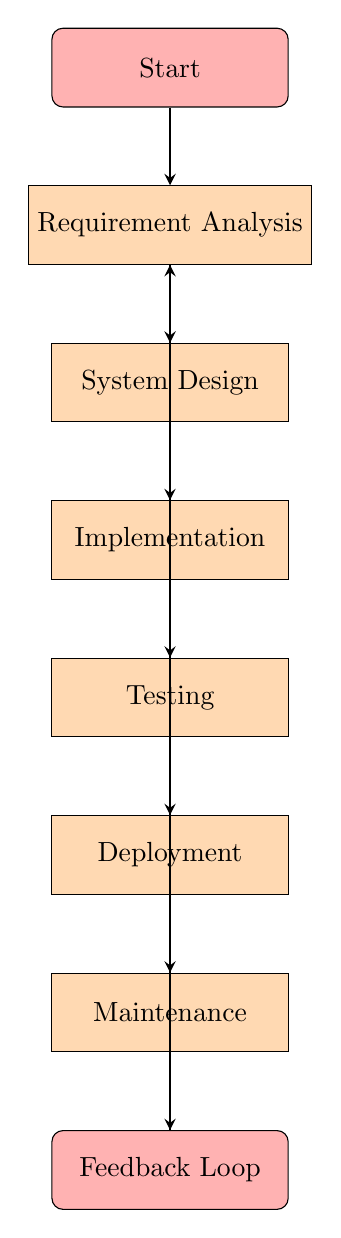
\begin{tikzpicture}[
            node distance=2cm,
            auto,
            startstop/.style={
                rectangle, 
                rounded corners, 
                minimum width=3cm, 
                minimum height=1cm,
                text centered, 
                draw=black, 
                fill=red!30
            },
            process/.style={
                rectangle, 
                minimum width=3cm, 
                minimum height=1cm, 
                text centered, 
                draw=black, 
                fill=orange!30
            },
            arrow/.style={
                thick, 
                ->, 
                >=stealth
            }
        ]
            % Define nodes
            \node[startstop] (start) {Start};
            \node[process, below of=start] (analysis) {Requirement Analysis};
            \node[process, below of=analysis] (design) {System Design};
            \node[process, below of=design] (implementation) {Implementation};
            \node[process, below of=implementation] (testing) {Testing};
            \node[process, below of=testing] (deployment) {Deployment};
            \node[process, below of=deployment] (maintenance) {Maintenance};
            \node[startstop, below of=maintenance] (feedback) {Feedback Loop};
            
            % Draw edges
            \draw[arrow] (start) -- (analysis);
            \draw[arrow] (analysis) -- (design);
            \draw[arrow] (design) -- (implementation);
            \draw[arrow] (implementation) -- (testing);
            \draw[arrow] (testing) -- (deployment);
            \draw[arrow] (deployment) -- (maintenance);
            \draw[arrow] (maintenance) -- (feedback);
            \draw[arrow] (feedback) -- (analysis);
        \end{tikzpicture}
    \end{center}
    \vspace{0.5cm}
    \begin{itemize}
        \item \textbf{Start:} Initiation of the project.
        \item \textbf{Requirement Analysis:} Gathering and analyzing project requirements.
        \item \textbf{System Design:} Designing the system architecture based on requirements.
        \item \textbf{Implementation:} Developing the system according to design specifications.
        \item \textbf{Testing:} Verifying that the system meets all requirements.
        \item \textbf{Deployment:} Launching the system to the production environment.
        \item \textbf{Maintenance:} Ongoing support and updates post-deployment.
        \item \textbf{Feedback Loop:} Continuously improving the system based on user feedback.
    \end{itemize}
\end{frame}

% Additional Slides
\section{Conclusion}
\begin{frame}{Conclusion}
    \begin{itemize}
        \item Summary of key points
        \item Future work
        \item Q\&A
    \end{itemize}
\end{frame}

\end{document} 